% compile using the following sequence of commands:
% pdflatex writeup
% bibtex writeup
% pdflatex writeup
% pdflatex writeup

% basic setup:
\documentclass[12pt, titlepage]{article}
\usepackage[utf8]{inputenc}
\usepackage[letterpaper, margin=1in]{geometry}
\usepackage{setspace}
\usepackage{amsmath}
\usepackage{graphicx}
\graphicspath{{./images/}}

% set up bibliography:
\usepackage[backend=bibtex, style=phys]{biblatex}
\addbibresource{citations.bib}

% change title sizes:
\usepackage{titlesec}
\titleformat*{\section}{\large\bfseries}
\titleformat*{\subsection}{\bfseries}

% change table of contents formatting:
\usepackage{tocloft}
\renewcommand{\cfttoctitlefont}{\large\bfseries}
\renewcommand{\cftsecfont}{\normalsize}
\renewcommand{\cftsubsecfont}{\normalsize}

% title page information:
\title{\Large Nucleation and Growth During the Crystalization \\
		of Amorphous Te Thin Films \\
		\bigskip
	\normalsize MSE 130: Experimental Materials Science and Design}
\author{\normalsize Jonathan Lee \\
	\normalsize Department of Materials Science and Engineering \\
	\normalsize University of California, Berkeley}
\date{\normalsize September 28th, 2020}

\begin{document}

\maketitle

\doublespacing

\setcounter{page}{2}

\tableofcontents

\newpage

\section{Abstract}

\section{Introduction}

novel electronic devices such as flexible displays will require the fabrication of semiconductors on noncrystalline substrates...the low melting points of such substrates (such as polymers etc) means that such processes must function on a low thermal budget...the semiconductor tellurium (Te) is an attractive candidate due to its relatively low melting point (449.5 degrees C)...this allows it to be deposited amorphously at low temperature, after which it may be crystallized near room temperature...additionally, the narrow band gap of bulk Te (0.32 eV) allows for straightforward bandgap engineering through electron confinement...depositing and crystallizing Te in a thin film allows its bandgap to be tuned to optimum values for a given application, such as FETs

the amorphous-deposition-crystallization manufacturing process may be understood in the context of classical Becker-Doering nucleation theory, which models the physical system as a distribution of atomic clusters.  The free energy change ($\Delta G$) of such a cluster is:
%
	\begin{equation}
		\Delta G(i) \approx -g_{c \rightarrow a}i + \gamma i^{2/3}
	\label{eqn:deltaG}
	\end{equation}
%
where $i$ is the number of atoms in the cluster, -$g_{c \rightarrow a}$ is the atomic free energy of the amorphous-to-crystalline transition, and $\gamma$ is a factor convolving the cluster surface energy and the surface-area-to-volume ratio.  Becker-Doering theory then uses steady-state and detailled-balance assumptions in order to derive the area nucleation rate $\dot{N}$:
%
	\begin{equation}
		\dot{N} \approx \dot{N_0} 
		\exp\left[-\frac{\Delta E_{attach} + \Delta G(i_c)}{k_T T}\right]
	\label{eqn:N_dot}
	\end{equation}
%
where $i_c$ is the critical cluster size and $\Delta E_{attach}$ is the activation energy for an atom to jump across the amorphous-crystalline interface.  The assumption of a spherical nucleus (Equation \ref{eqn:deltaG}) motivates a critical nucleation energy of $\Delta G(i_c) = \frac{4 \gamma^3}{27g_{c \rightarrow a}^2}$.  The units of $\dot{N}$ are $m^{-2}s^{-1}$.

The crystallization process may be additionally described through Johnson-Mehl-Avrami-Kolmogorov theory in the 2D limit, wherein a nucleus grows to span the thickness of the film faster than the next nuclus can appear.  In such a limit, the area fraction transformed ($\alpha$) is described by the JMAK equation:
%
	\begin{equation}
		\alpha = 1 - \exp
		\left[ -\frac{\pi}{3}\dot{N}v^2t^3 \right]
	\label{eqn:alpha}
	\end{equation}
%
where the growth velocity (in units of $\frac{m}{s}$) follows an Arrhenius dependence:
%
	\begin{equation}
		v \approx v_0 \exp \left[ - \frac{\Delta E_{attach}}{k_B T} \right]
	\label{eqn:v}
	\end{equation}
%
Finally, JMAK theory produces an expression for the average number of grains nucleated per unit area:
%
	\begin{equation}
		\rho = \left(\frac{3}{\pi}\right)^{\frac{1}{3}}
		\Gamma \left[ \frac{4}{3} \right]
		\left( \frac{\dot{N}}{v} \right)^{\frac{2}{3}}
	\label{eqn:rho}
	\end{equation}
%
where $\Gamma \left[ \frac{4}{3} \right] \approx 0.8929795...$ is the Euler Gamma function.

Taken collectively, B-D theory and JMAK theory yield a straightforward method for calculating $\dot{N}$, $v$, and their associated activation energies and prefactors.  An amorphous Te thin film may be monitored during its anneal in order to measure the crystalline area fraction as a function of time, which may be fitted to Equation \ref{eqn:alpha} to calculate $\dot{N}v^2$.  Afterwards, the grain density may be assessed and Equation \ref{eqn:rho} may be employed to calculate $\dot{N}/v$.  These values may be trivially solved for $\dot{N}$ and ${v}$.

Repeating the procedure at different annealing temperatures allows the Arrhenius forms (Equations \ref{eqn:v} and \ref{eqn:N_dot}) to be fit, thus providing estimates of the activation energies governing nucleation and growth in the low-temperature Te manufacturing process.

The equations presented in this section represent the core results of B-D and JMAK theory.  For a detailled discussion of their derivations and assumptions, as well as a demonstration of the validity of the 2D limit, see Reference \cite{chrzan:2020}.


\section{Experimental Procedure}

An Edwards 306 Thermal Evaporator was loaded with Te source pellets of 99.999\% purity from Sigma-Aldrich.  Te was deposited on a substrate at a deposition rate of approximately 10 \r{A}/sec.  Film thicknesses, as controlled by a quartz crystal microbalance, ranged from 4 to 20 nm.  Since the substrate was maintained at -80\textdegree{C}, the deposited film was amorphous, as later verified by x-ray diffraction.\cite{chrzan:2020}

Six deposited films were selected for experimental analysis.  Immediately after deposition, each film was heated to its target annealing temperature (10\textdegree{C}, 15\textdegree{C}, 20\textdegree{C}, 25\textdegree{C}, 30\textdegree{C}, or 35\textdegree{C}).  Optical microscopy was used to observe the crystallization at an imaging rate of 2.87 frames/sec,\cite{chrzan:2020} with the intent that these data be used to assess the area fraction transformed (Equation \ref{eqn:alpha}).

After annealing, the samples were allowed to return to room temperature, then examined via transmission electron microscope.  Bright field and dark field images of a 140 \textmu{m} x 105 \textmu{m} region were obtained, with the intent that they be used to determine the films' grain density (Equation \ref{eqn:rho}).  Additional images of a zoomed-in 140 \textmu{m} x 105 \textmu{m} region were collected for the 20\textdegree{C}, 25\textdegree{C}, 30\textdegree{C}, and 35\textdegree{C} samples.\cite{chrzan:2020}  These higher-temperature films were observed to possess finer microstructures, so the additional images were to serve as a backup in case the grain density proved too difficult to quantify at the original magnification.


\section{Results}

obtaining and fitting fraction transformed curves

assessing grain density from microstructural images

calculating parameters and estimating free energies/critical nuclei

Data processing took place in three stages: (1) the conversion of the optical microscopy videos to $\alpha$-curves for the fitting of Equation \ref{eqn:alpha}; (2) the determination of grain densities from the electron microscopy images for the fitting of Equation \ref{eqn:rho}; and (3) the use of the fitting results to calculate the parameters governing the Te manufacturing process.  Each of these three stages is treated in a subsection below.  All code involved in the calculations may be found in the Github repository linked in Appendix A.

\subsection{JMAK Equation Fitting to Determine $\dot{N}v^2$}

The optical microscopy videos collected during the films' annealing stage were observed to consist of (1) dark regions corresponding to the amorphous phase and (2) regions of greater intensity correponding to the crystalline phase.  Each frame could therefore be converted to its corresponding $\alpha$-value by calculating its average intensity, then normalizing the resulting data to the maximum and minimum average intensities observed during the anneal ($\alpha = 1$ and $\alpha = 0$, respectively).  Several abrupt jumps in average intensity were recorded; this was attributed to automatic intensity rescaling from the imaging system itself.  Fortunately, none of these jumps occured during the main transition region of the curves, allowing the model to be cleanly fit to a rescaled subset of the data.  The selected regions and assigned $\alpha = 0$ rescaling values for each temperature is noted in Figure \ref{fig:jmak_2} of Appendix B.

The actual data fit employed a modified version of the JMAK equation:
%
	\begin{equation}
	\alpha =
	\begin{cases}
		0 & t < t_0 \\
		1 - \exp \left[ -\frac{\pi}{3} \dot{N} v^2 (t-t_0)^3 
			\right] & t_0 \leq t
	\end{cases}
	\label{eqn:jmak_modified}
	\end{equation}
%
where the fitting parameter $t_0$ is introduced to reflect variation in the annealing time \cite{chrzan:2020} and the piecewise nature enforces physicality (i.e. $\alpha = 0$ for $t < t_0$).  The nonlinear fitting was performed with the Python package \textit{lmfit}, which also estimated the standard error associated with each of the fitting parameters.\cite{lmfit}  The results of this fitting are summarized in Table \ref{table:data_results} and visualized in Figure \ref{fig:jmak_1}.
	

	\begin{figure}[h]
		\centering
		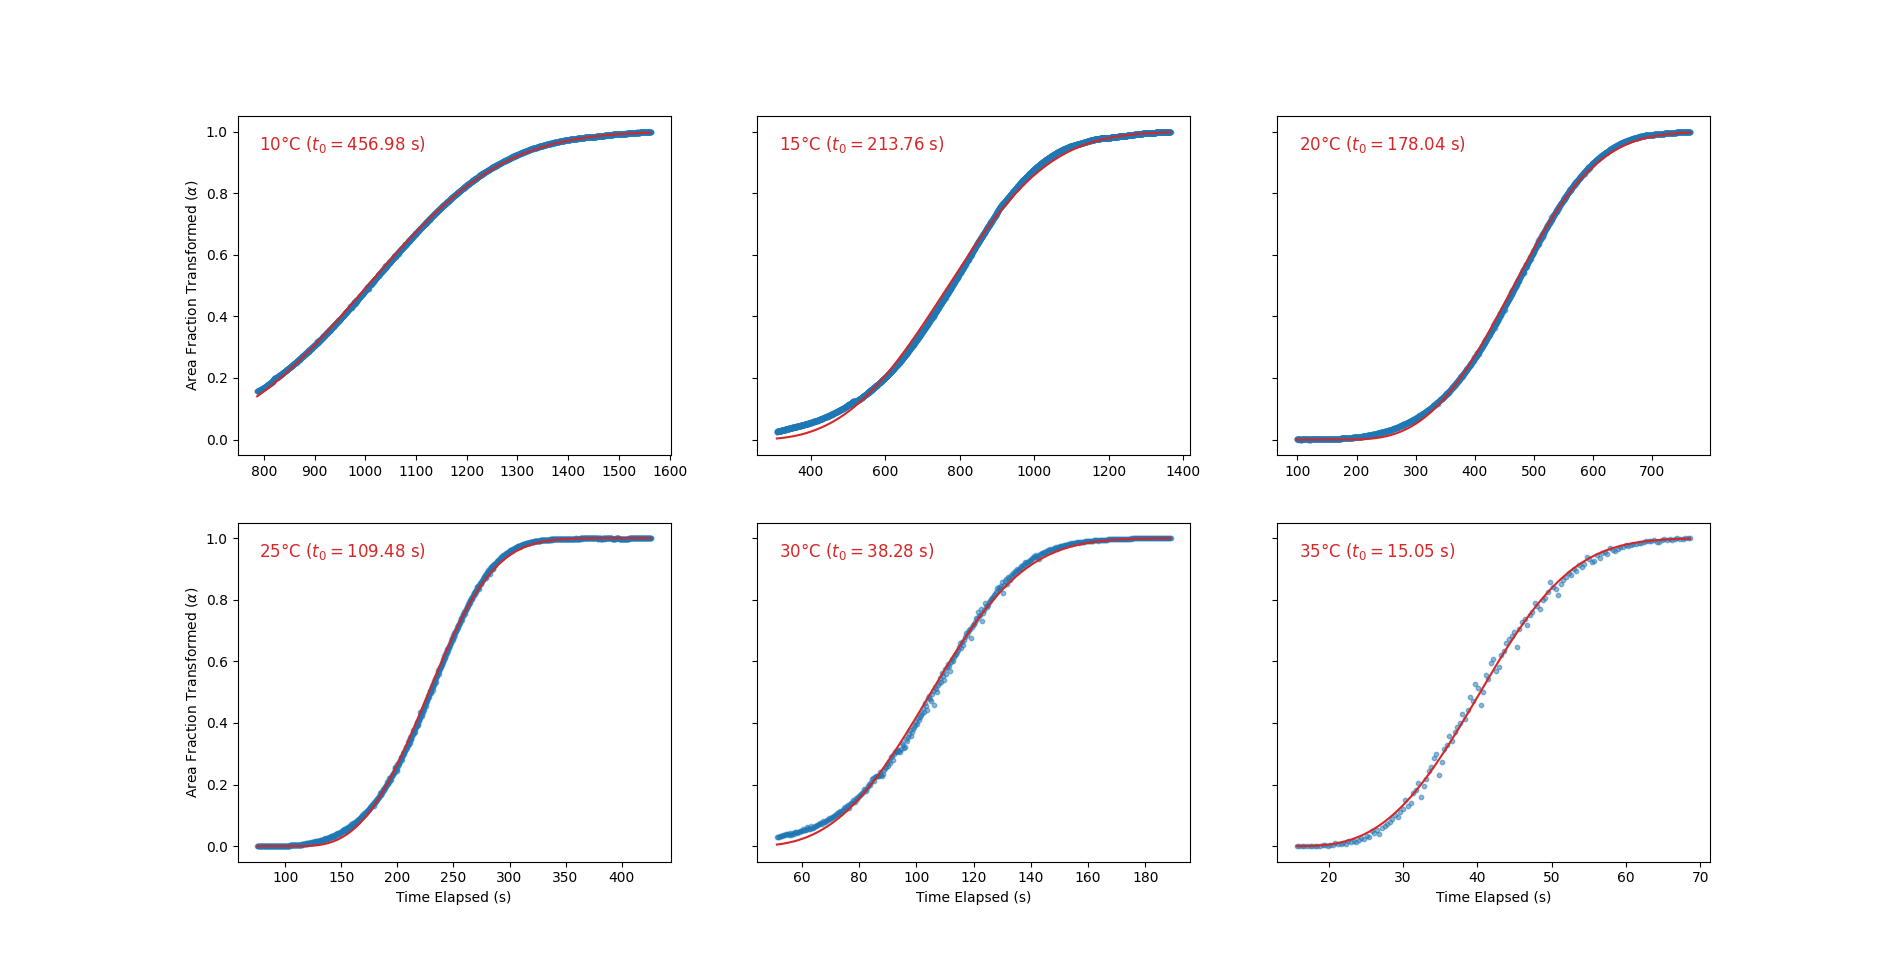
\includegraphics[width=1.0\linewidth]{jmak_1.png}
		\caption{Results of fitting the JMAK equation (Equation \ref{eqn:jmak_modified}) to the rescaled transformation data derived from the sample transformation videos.  In the region of the transformation, the model appears to fit the data closely.  The data displayed here are a subset of the entire $\alpha$-curves, which contained jumps attributed to lighting adjustments; the full data may be found in Figure \ref{fig:jmak_2} in Appendix B.}
		\label{fig:jmak_1}
	\end{figure}

\subsection{Microstructural Image Processing to Determine $\dot{N}/v$}

Using the image analysis procedures described in References \cite{chan:2020} and \cite{campbell:2018} as a loose guide, an rudimentary algorithm was developed in order to process the samples' electron microscopy images and count grains in a consistent manner.  For simplicity, counts were only performed for the 140-\textmu{m} images.  Given the dark field image, the bright field image, and a manual input parameter denoting the minimum detectable grain radius ($r_{min}$), the algorithm performs the following operations using the Python package \textit{scikit-image}\cite{skimage}:

\begin{enumerate}

	\item Both images are converted to greyscale, after which a Sobel filter is applied to the bright field to calculate its local gradient.  This produces maps where bright regions correspond to possible grain boundaries.

	\item The the two maps are adjusted such that the middle 95\% of pixel intensities are mapped across the intensity range [0, 1], so as to increase contrast for the majority of the map pixels.

	\item The maps are averaged and the results inverted.  In the resulting grain map, bright regions correspond to probable grain locations, while dark regions correspond to boundaries.  Combining the maps is necessary due to the observation that certain grain boundaries appear only in one of the maps.

	\item Gaussian smoothing is applied to remove some noise, after which gaussian sharpening is applied to increase boundary contrast.

	\item Multiple-otsu thresholding is used to sort the pixels into four different intensity bins; this was observed to isolate grains in the fourth bin, even in the presence of faint grain boundaries (assumed to be low-angle grain boundaries).  The fourth bin therefore produces a binarized image of the grains.

	\item A "weighted opening" is executed upon the binarized image.  The pixels are eroded with a radius of $r_{min}$ before being dilated with a radius of $r_{min} / 2$.  This has the effect of eliminating all pixels upon repeated cycling.  Intermediate results are stacked, thereby creating a heatmap of the number of opening cycles required to eliminate any pixel.  This has the effect of replacing each pixel with the distance to the nearest grain boundary, albeit in a way that is meant to promote round grains and smooth heatmap topology.

	\item The local maxima of the heatmap (to within radius $r_{min}$) are counted as the locations of grains.

	\item For diagnostic purposes, the watershed algorithm is then used to produce a grain map and assess the quality of the algorithm's result.

\end{enumerate}

This process is illustrated in Figure \ref{fig:algo_ex} for the 20 \textdegree{C} sample, with comparable figures for all other temperatures contained in Appendix B.  The resulting grain densities and $\dot{N}/v$ values, as calculated using Equation \ref{eqn:rho}, are included in Table \ref{table:data_results}.

	\begin{figure}[h]
		\centering
		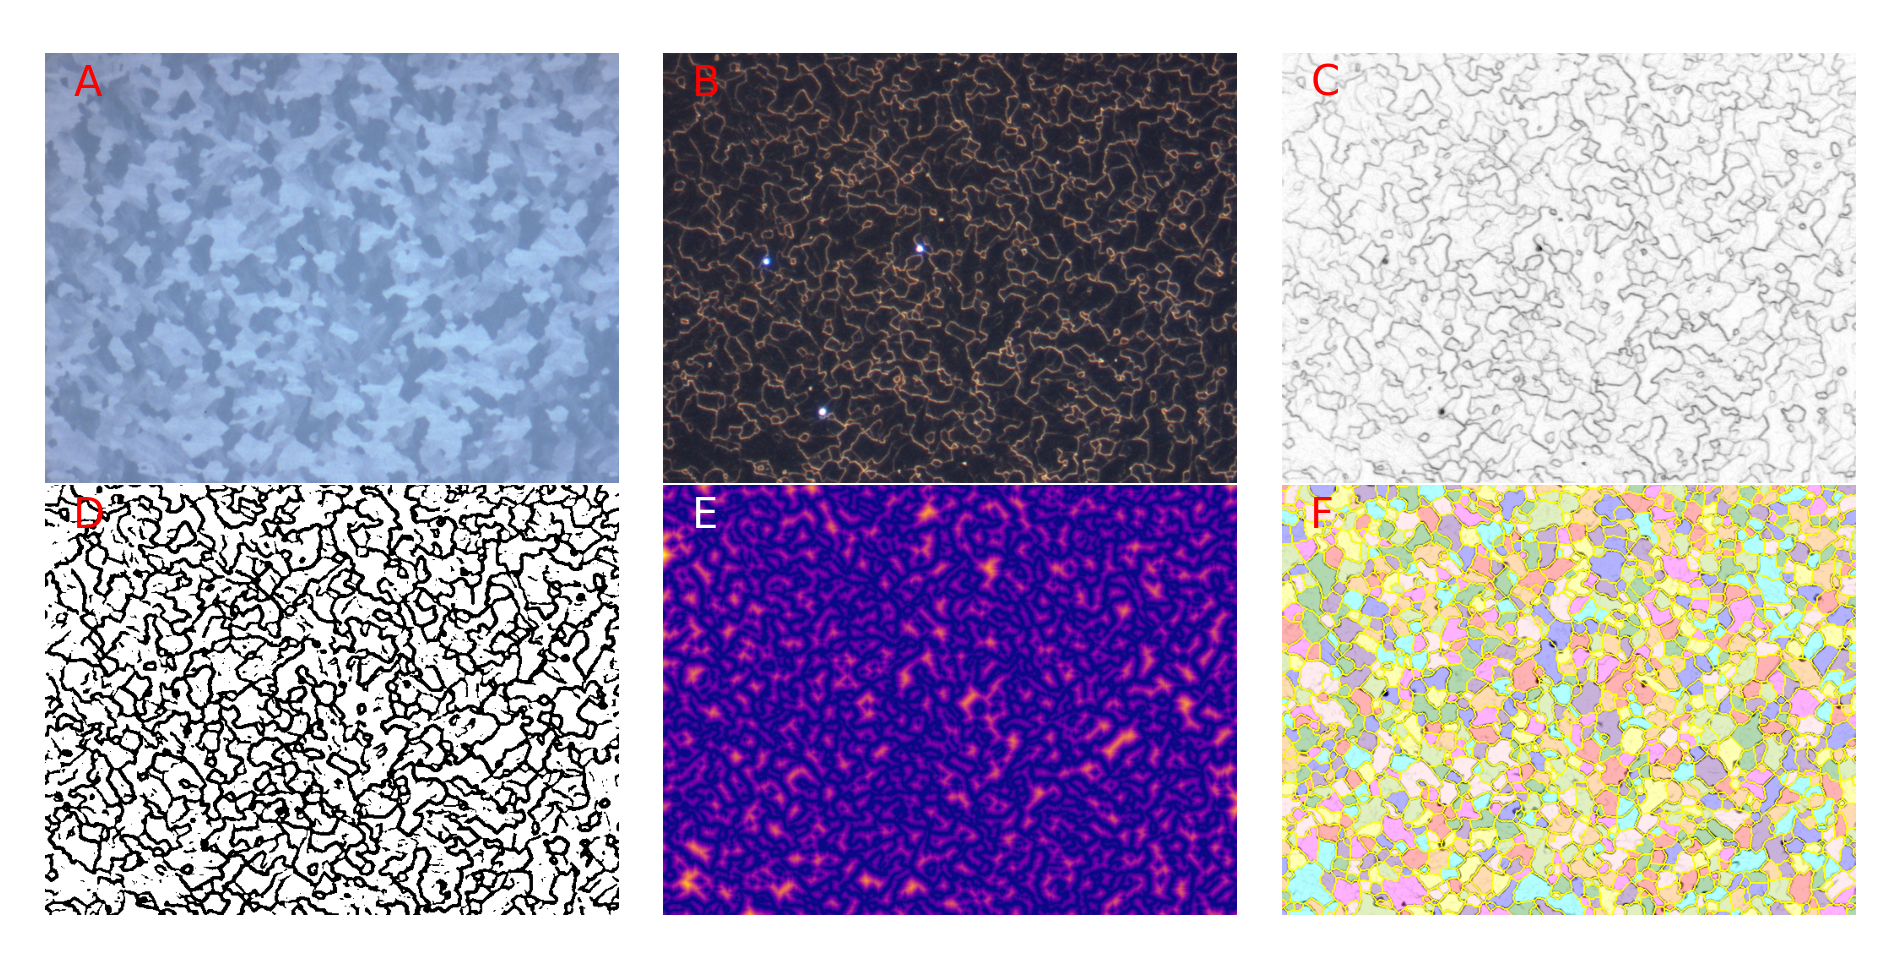
\includegraphics[width=1.0\linewidth]{microstructure_20C.png}
		\caption{Intermediate results of the grain-counting algorithm for the 20 \textdegree{C} anneal. (A) Bright field image; (B) dark field image; (C) merged bright/dark field map; (D) grains as the fourth bin of multiple-otsu thresholding; (5) ``heatmap'' generated by the ``weighted opening'' loop; (6) final grain map.}
		\label{fig:algo_ex}
	\end{figure}

A discussion of the quality of the grain-counting algorithm, particularly with respect to the decision not to attempt to quantify its error, is deferred to Section 5.

	\begin{table}[h!]
	\centering
	\begin{tabular}{|c c c c c c c|} 
	\hline
		T (\textdegree{C}) & $\dot{N}v^2 (s^{-3})$ & $\sigma_{\dot{N}v^2}(s^{-3})$ & $t_0 (s)$ & $\sigma_{t_0}$ & $\rho (m^{-2})$ & $\dot{N}/v (m^{-3})$ \\ 
	\hline
		10 & 4.023e-9 & - & 456.98 & - & 3.396e+10 & 7.588e+15\\ 
		15 & 3.845e-9 & - & 213.76 & - & 5.210e+10 & 1.442e+16\\
		20 & 2.773e-8 & 1.115e-10 & 178.04 & 0.427 & 8.469e+10 & 2.989e+16\\
		25 & 3.978e-7 & 2.507e-09 & 109.48 & 0.259 & 9.048e+10 & 3.300e+16\\
		30 & 2.211e-6 & 3.198e-08 & 38.28 & 0.333 & 1.386e+11 & 6.256e+16\\
		35 & 4.069e-5 & 9.426e-7 & 15.05 & 0.201 & 2.644e+11 & 1.648e+17\\
	\hline
	\end{tabular}
		\caption{Summary of results from $\alpha$-fitting (Subsection 4.1) and grain-counting (Subsection 4.2).  For 10 \textdegree{C} and 20 \textdegree{C}, standard errors could not be calculated by \textit{lmfit}.}
	\label{table:data_results}
	\end{table}

\subsection{Calculation of Crystallization Parameters}

Throughout the following calculations, the standard errors of $\dot{N}v^2$ were propagated according to a well-known formula:

	\begin{equation}
		f(a_1, a_2, ...) \rightarrow \sigma^2_f = \sum_i \left( \frac{\partial f}{\partial a_i} \right)^2 \sigma^2_{a_i}
		\label{eqn:se}
	\end{equation}

From the values of $\dot{N}v^2$ and $\dot{N}/v$ in Table \ref{table:data_results}, $\dot{N}$ and $v$ were obtained for each temperature.  These values are summarized in Table \ref{table:nv_results}:

	\begin{table}[h!]
	\centering
	\begin{tabular}{|c c c c c |} 
	\hline
		T (\textdegree{C}) & $\dot{N}(m^{-2}s^{-1})$ & $\sigma_{\dot{N}}(m^{-2}s^{-1})$ & $v (m/s)$ & $\sigma_{v} (m/s)$ \\ 
	\hline
		10 & 6.141e+07 & - & 8.093651e-09 & -\\ 
		15 & 9.281e+07 & - & 6.436233e-09 & -\\
		20 & 2.915e+08 & 3.907e5 & 9.753040e-09 & 1.307e-11\\
		25 & 7.567e+08 & 1.590e6 & 2.292838e-08 & 4.817e-11\\
		30 & 2.053e+09 & 9.898e6 & 3.281534e-08 & 1.582e-10\\
		35 & 1.034e+10 & 1.983e7 & 6.273605e-08 & 4.843e-10\\
	\hline
	\end{tabular}
		\caption{$\dot{N}$, $v$, and associated standard errors, as calculated from the results in Table \ref{table:data_results}.} 
	\label{table:nv_results}
	\end{table}

These data were then fit to their respective Arrhenius models in ln-versus-$1/T$ coordinates using linear regression so as to estimate the corresponding prefactors and activation energies.  The linear fit is illustrated in Figure \ref{fig:linear_fits}, while the calculated parameters and corresponding standard errors from the linear regression are summarized in Table \ref{table:parameter_results}.  The standard errors of $\dot{N}$ and $v$ were not propagated into this step; the uncertainties stem from the linear regression itself.

	\begin{table}[h!]
	\centering
	\begin{tabular}{|c | c | c | c | c |} 
		\hline
		\textbf{Parameter} & $\Delta G(i_c) + \Delta E_{attach}$ (eV) & $\Delta E_{attach}$ (eV) & $\dot{N_0}$ ($m^{-2}s^{-1}$) & $v_0$ (m/s) \\ 
		\hline
		\textbf{Value} & 1.536 & 0.682 & 8.646e34 & 7432 \\
		\textbf{$\sigma$} & 0.136 & 0.117 & 4.615e35 & 34307 \\
		\hline
	\end{tabular}
		\caption{Arrhenius parameters found by performing linear fits on $\ln{\dot{N}}$ and $\ln{v}$ with respect to $1/T$ (see Figure \ref{fig:linear_fits}).}
	\label{table:parameter_results}
	\end{table}

	\begin{figure}[h]
		\centering
		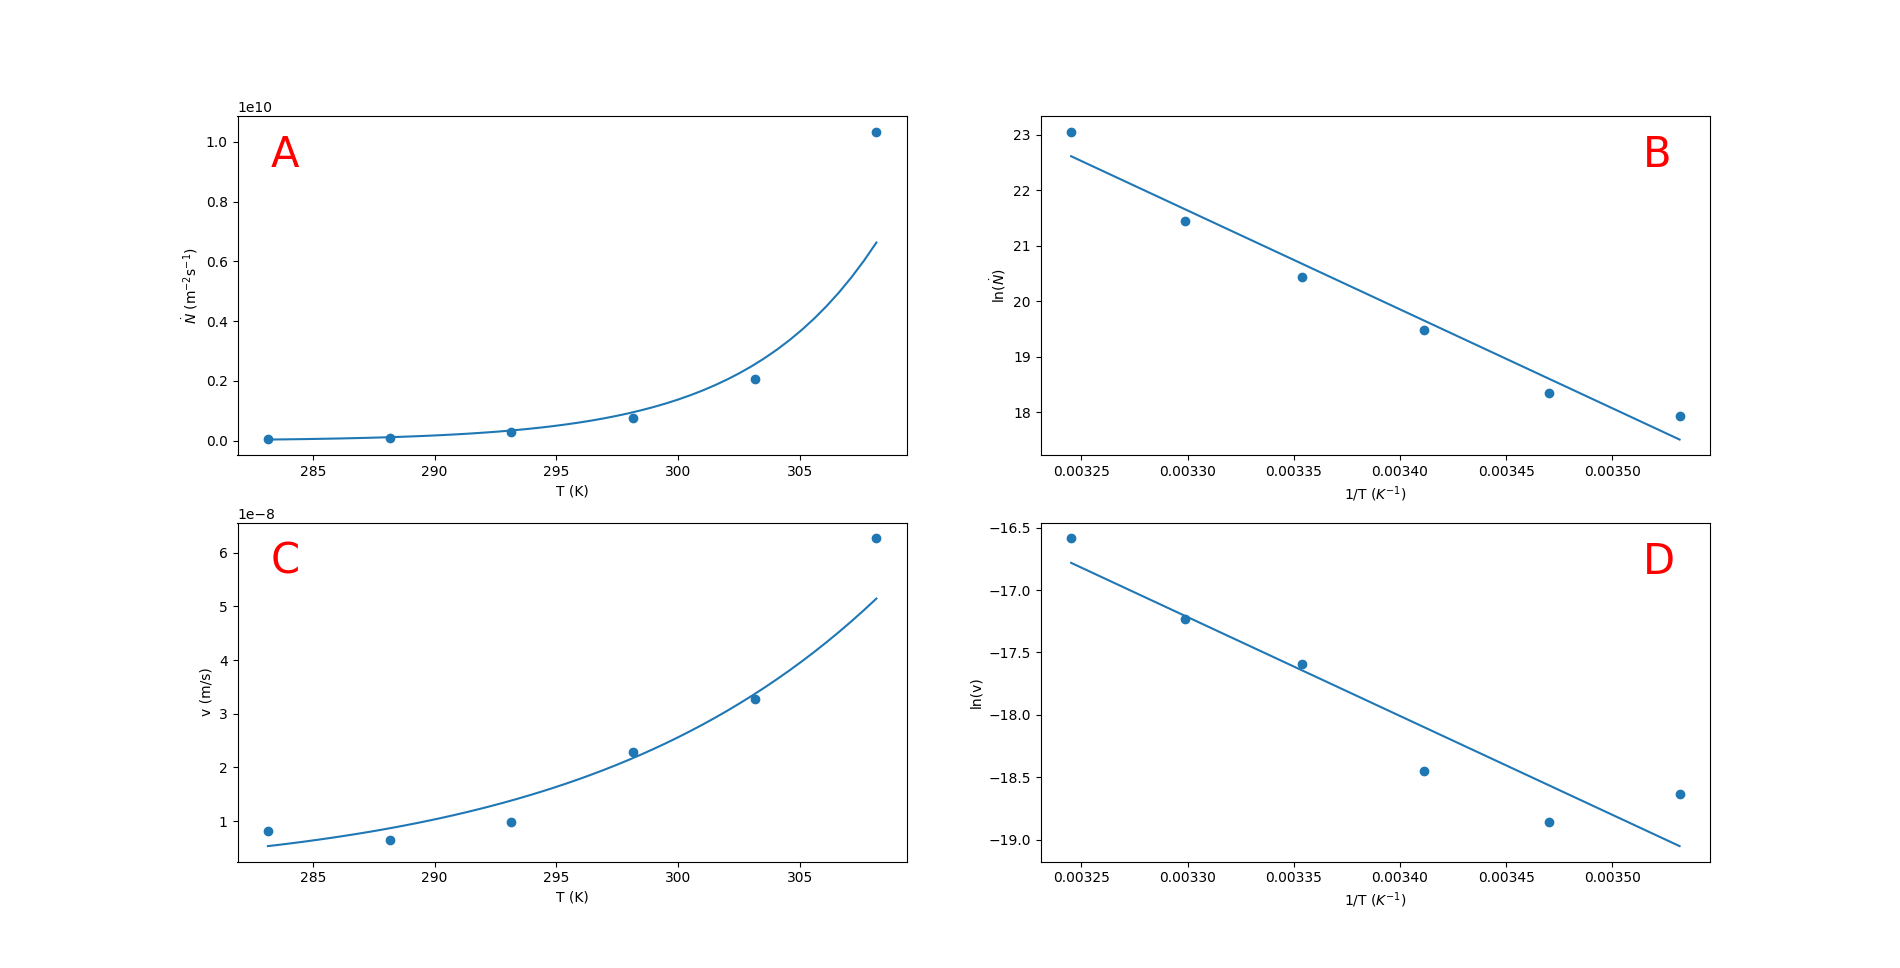
\includegraphics[width=1.0\linewidth]{linear_fits.png}
		\caption{Linear fits of $\ln{\dot{N}}$ and $\ln{v}$ with respect to $1/T$, used to find the Arrhenius parameters in Table \ref{table:parameter_results}.  For $\dot{N}$, $R^2 = 0.970$, while for $v$, $R^2 = 0.894$.}
		\label{fig:linear_fits}
	\end{figure}

Subtracting the activations energies yields the free energy change per atom of the critical nucleus, $\Delta G(ic) = 0.853$ eV, with a standard error of 0.696 eV.

The next logical step is to estimate the critical cluster size ($i_c$) and the enthalpy of crystallization ($-g_{c \rightarrow a}$); however, this requires knowledge of the $\gamma$-factor that appears in Equation \ref{eqn:deltaG}.  An extremely-loose estimate may be obtained by the Materials Project: the average surface free energy of a Te Wulff crystal ($\gamma_s = 0.11 J/m^2$) may be taken as an upper bound for the possible energy of the crystalline-amorphous interface.\cite{jain:2018}

In order to convert from this surface free energy to the $\gamma$-factor of Equation \ref{eqn:deltaG}, a spherical critical nucleus is assumed, for which the nucleation barrier is typically calculated in terms of the critical radius ($r_c$):

\begin{equation}
	\Delta G(r_c) = -\frac{4}{3}\pi r_c^3 \Delta G_v + 4 \pi r_c^2 \gamma_s
	\label{eqn:rc}
\end{equation}

Recognizing that $V_c = \frac{4}{3}\pi r_c^3 = \Omega i_c$ where the atomic volume $\Omega = 35.031$ $\si{\angstrom}^3$, the expression $r_c = \left( \frac{3\Omega i_c}{4\pi} \right)^{1/3}$ may be obtained, yielding the following alternate form of Equation \ref{eqn:rc}:

\begin{equation}
	\Delta G(r_c) = -\Delta G_v \Omega i_c + 4 \pi \gamma_s \left( \frac{3\Omega i_c}{4\pi} \right)^{2/3} 
	\label{eqn:rc_ic}
\end{equation}

A comparison with Equation \ref{eqn:deltaG} reveals that the desired $\gamma$-factor may be calculated as $\gamma = 4 \pi \gamma_s \left( \frac{3\Omega}{4\pi} \right)^{2/3}$.  Recalling that the free energy of the spherical critical nucleus may be expressed as $\Delta G(i_c) = \frac{4 \gamma^3}{27 g^2_{c \rightarrow a}}$, the energy difference between amorphous and crystalline phases may be calculated as $g_{c \rightarrow a} = \sqrt{\frac{4 \gamma^3}{27 \Delta G(i_c)}}$, while the critical nucleus size is obtained as $i_c = \frac{2 \gamma}{3 g_{c \rightarrow a}}$.

Following these equations, the upper surface energy limit of $\gamma_s = 0.11 J/m^2$ yields $\gamma = 0.356$ eV, $g_{c \rightarrow a} = 0.088$ eV, and a critical cluster size $i_c = 2.683$ atoms.  By design, these values represent a lower limit; the critical cluster size may be made arbitrarily large by decreasing the estimate of $\gamma$ towards 0 eV.  This relationship is illustrated in Figure \ref{fig:cluster_size}.

	\begin{figure}[h]
		\centering
		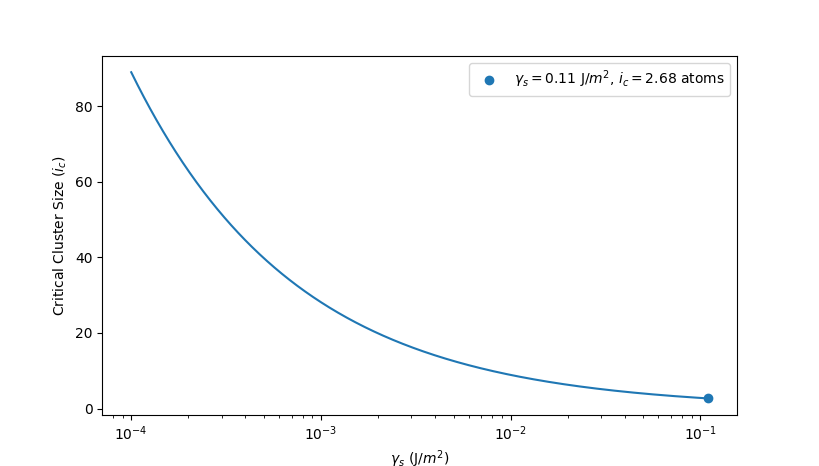
\includegraphics[width=1.0\linewidth]{cluster_size.png}
		\caption{Graph of the relationship between $i_c$ and $\gamma_s$.  By decreasing $\gamma_s$ towards 0, the critical cluster may be made arbitrarily large, highlighting the need to improve the estimate of the crystalline-amorphous surface energy.}
		\label{fig:cluster_size}
	\end{figure}


\section{Discussion}

discussion of validity of free energy and critical nuclei result

discussion of validity of grain counting algorithm

discussion of improvements to the estimation procedure and attempt to derive gamma

\subsection{Comments Upon Validity of Area Transformed Data}

As described in Subsection 4.1, the area fraction transformed ($\alpha$) was calculated for each optical frame simply as the average intensity of that frame.  The entire $\alpha$ curve for the sample was subsequently rescaled.  After this analysis was complete, however, it was observed that several of the videos comtain a faint lighting gradient, which may have negatively impacted the accuracy of the calculation.  Specifically, if the sample were improperly illuminated such that the crystalline regions received more or less light on average, then this would produce a systematic error in the results $\alpha$-curves.  Such a scenario becomes progressively more likely as the annealing temperature is lowered and the crystalline phase nucleates in a less-distributed manner.

A different analysis pipeline that addresses the issue would be to binarize and adaptively threshold each frame, thereby counting the fraction of pixels deemed ``bright enough'' to be crystalline based on local lighting conditions.  This, however, has the disadvantage of being sensitive to a dirtied optical lens; care would need to be taken to ignore pixels occluded by dirt or dust on the microscope. 

\subsection{Comments Upon Accuracy of Grain-Counting Algorithm}

Perhaps the most unsound decision made in this analysis was to avoid quantifying inaccuracies in the grain-counting algorithm of Subsection 4.2.  As shown in Figure \ref{fig:miscount}, the algorithm produces miscounts if it fails to find a local maximum for a given grain.  A more rigorous approach, such as that taken in Reference \cite{campbell:2018}, would involve aggressively overestimating the number of grains, after which a supplementary algorithm might be employed to merge adjacent watershed cells deemed similar enough to comprise a single grain.

The possibility of testing the algorithm against computer-generated training data was considered.  In this scenario, bright field and dark field images would be digitally generated for a variety of grain densities, then fed to the algorithm in order to quantify its standard error.  This error would then be translated to error in $\dot{N}/v$ and propagated through the remainder of the calculations.  The main obstacle to this analysis \textit{in silico} is that there is no way of guaranteeing that such artificial electron micrographs would possess qualities similar to real ones; the procedure would quantify the algorithm's error with respect to the sythetic data set only.

In this respect, the results of the grain-counting algorithm should only by viewed as a loose estimate, albeit with greator rigor and consistency than manual counting.

	\begin{figure}[h]
		\centering
		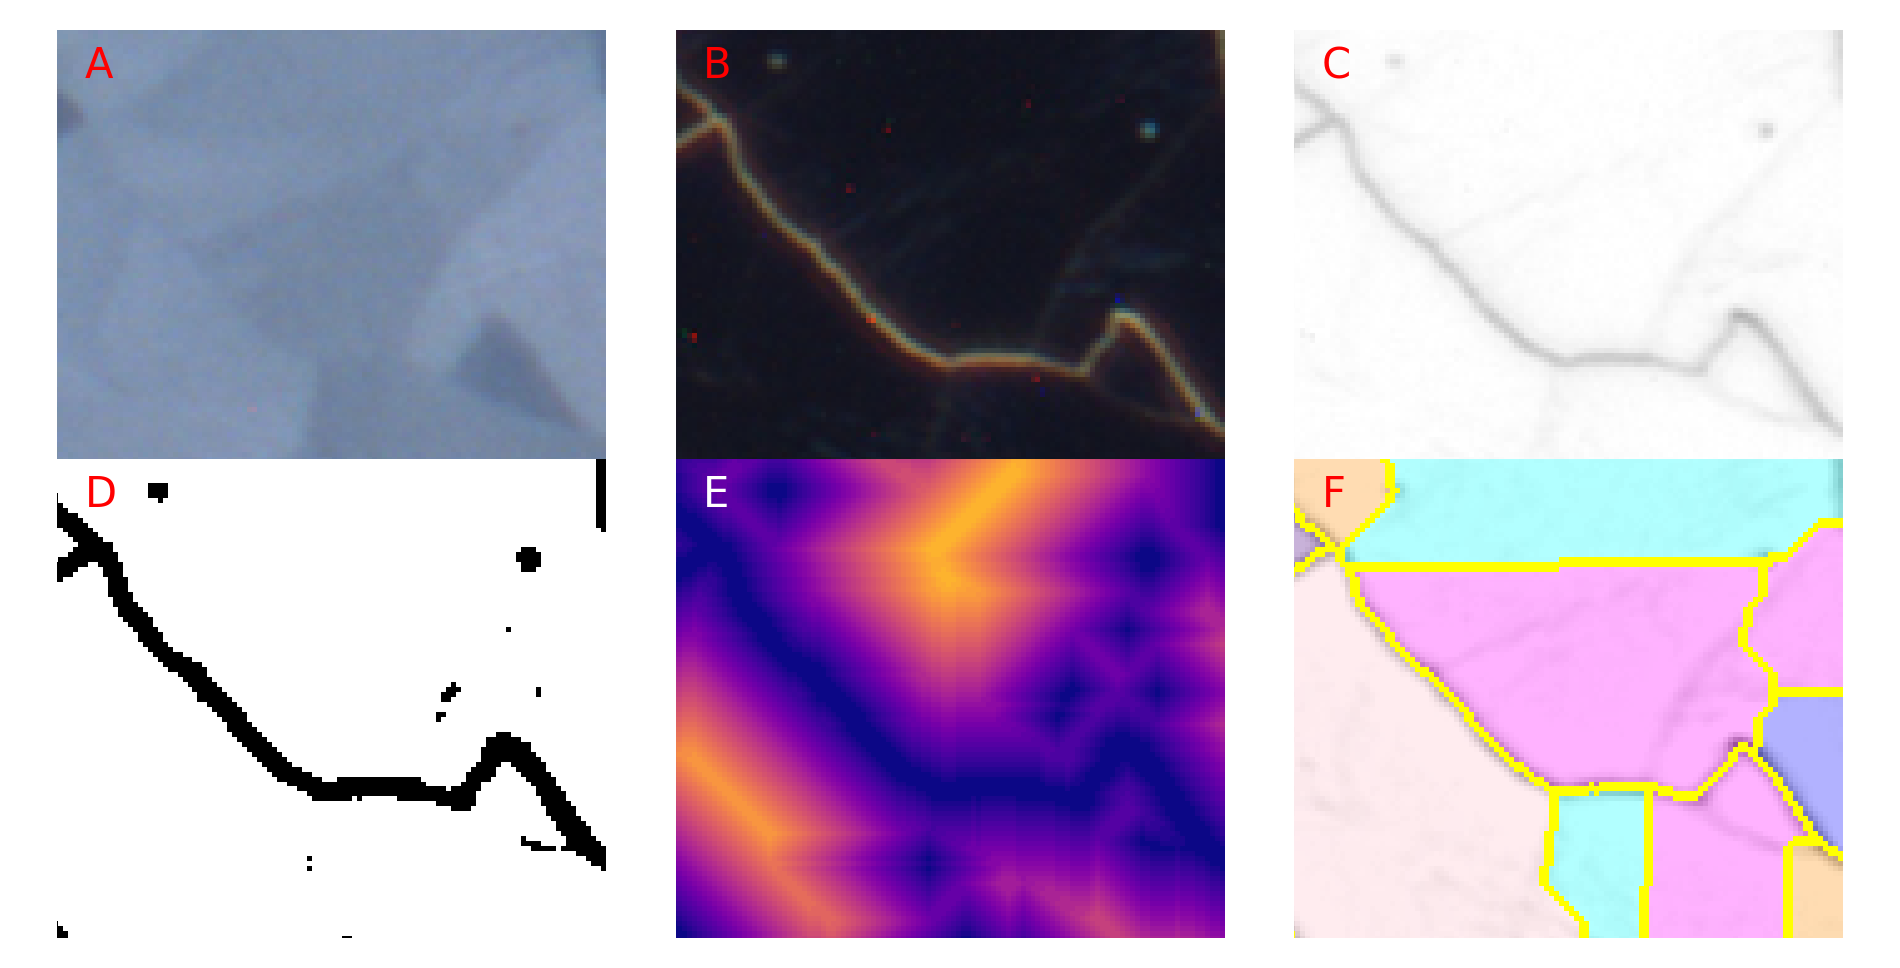
\includegraphics[width=1.0\linewidth]{miscount_10C.png}
		\caption{}
		\label{fig:miscount}
	\end{figure}

\subsection{Validity of Obtained Crystallization Parameters}

As evidenced by the graph in Figure \ref{fig:cluster_size}, the results of the parameter calculations of Subsection 4.3 do not truly yield an estimate for $g_{c \rightarrow a}$ and $i_c$, but rather a methodology for predicting them based on an estimate of $\gamma$.  From its lower limit of 2.683 atoms, the critical cluster size may be made arbitrarily large by changing the input $\gamma$, and a literature review yielded no methodology (beyond large-scale atomic simulations) for calculating the energy of the crystalline-amorphous interface.  These parameters should also be regarded with skepticism, given the assumption of a spherical nucleus with isotropic properties; in reality, Te manifests a trigonal crystal structure with a highly-anisotropic Wulff shape.  Refining the calculation to reflect these properties would likely require reengineering the Becker-Doering and JMAK results from the ground up.

Despite these reservations regarding the fundamental parameters of the crystalline-amorphous transformation, the Arrhenius laws for $\dot{N}$ and $v$ appear to fit the data moderately well, and as such may be used to predict the samples' annealing behavior.  The large standard errors of the prefactors in Table \ref{parameters_result} are a byproduct of fitting the data in $1/T$-ln coordinates; the actual coefficients of determination for the linear fit are $R^2_{\dot{N}} = 0.970$ and $R^2_v = 0.894$.  Most of the uncertainty appears to stem from the grain counts at 25 \textdegree{C} and 30 \textdegree{C}, which appear to be above and below the trend set by the other data, respectively.



\section{Conclusions}

\section{Acknowledgments}

\printbibliography[heading=bibnumbered]

\section{Additional Graphs}

	\begin{figure}[h]
		\centering
		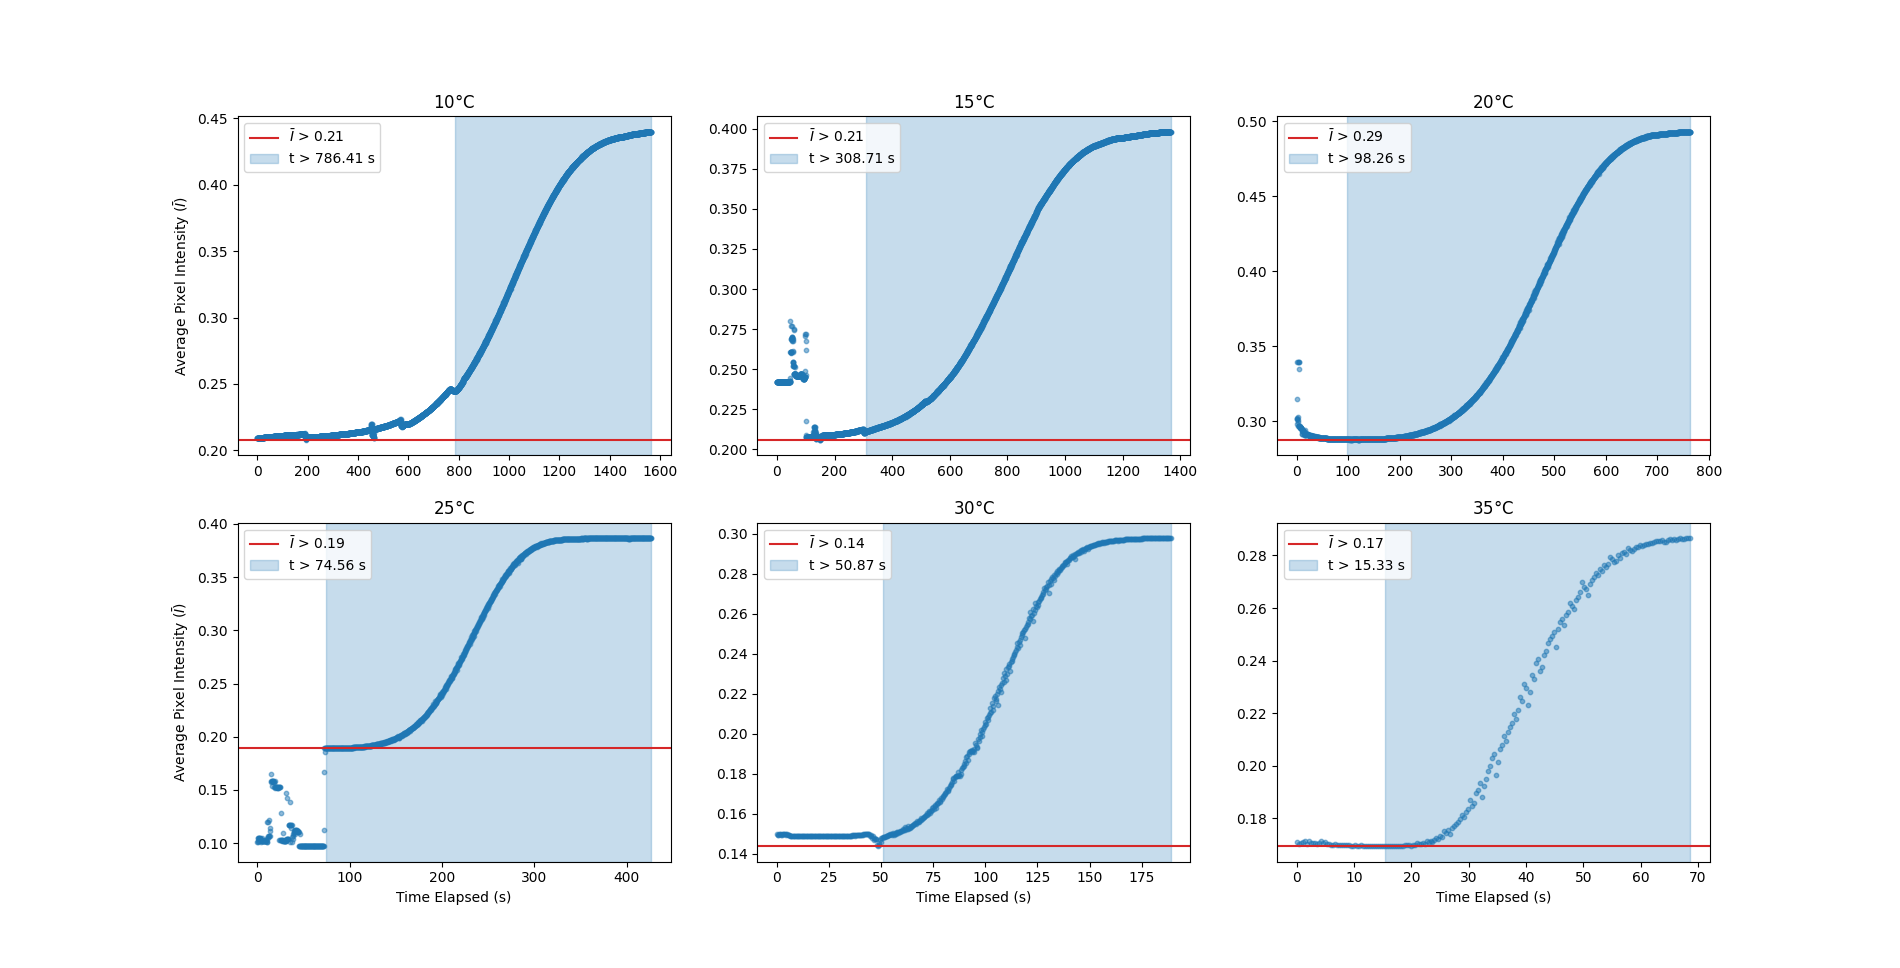
\includegraphics[width=1.0\linewidth]{jmak_2.png}
		\caption{}
		\label{fig:jmak_2}
	\end{figure}

	\begin{figure}[h]
		\centering
		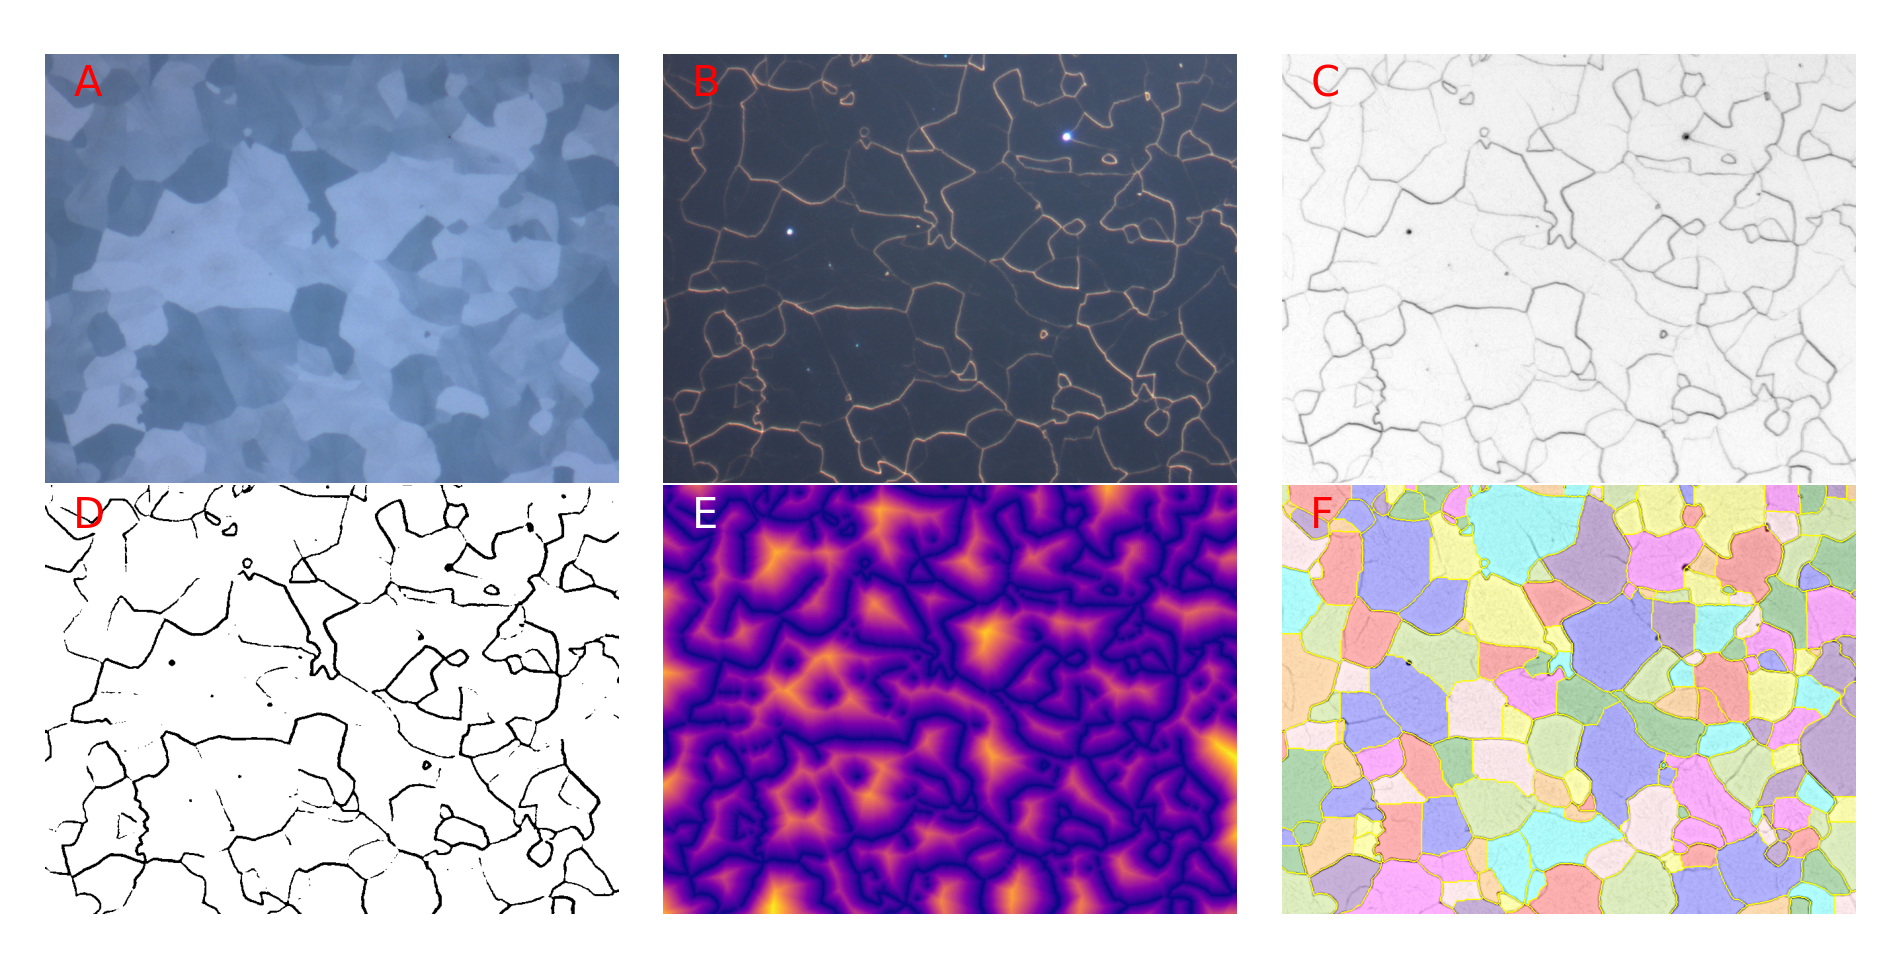
\includegraphics[width=1.0\linewidth]{microstructure_0C.png}
		\caption{}
		\label{fig:micro_0C}
	\end{figure}

	\begin{figure}[h]
		\centering
		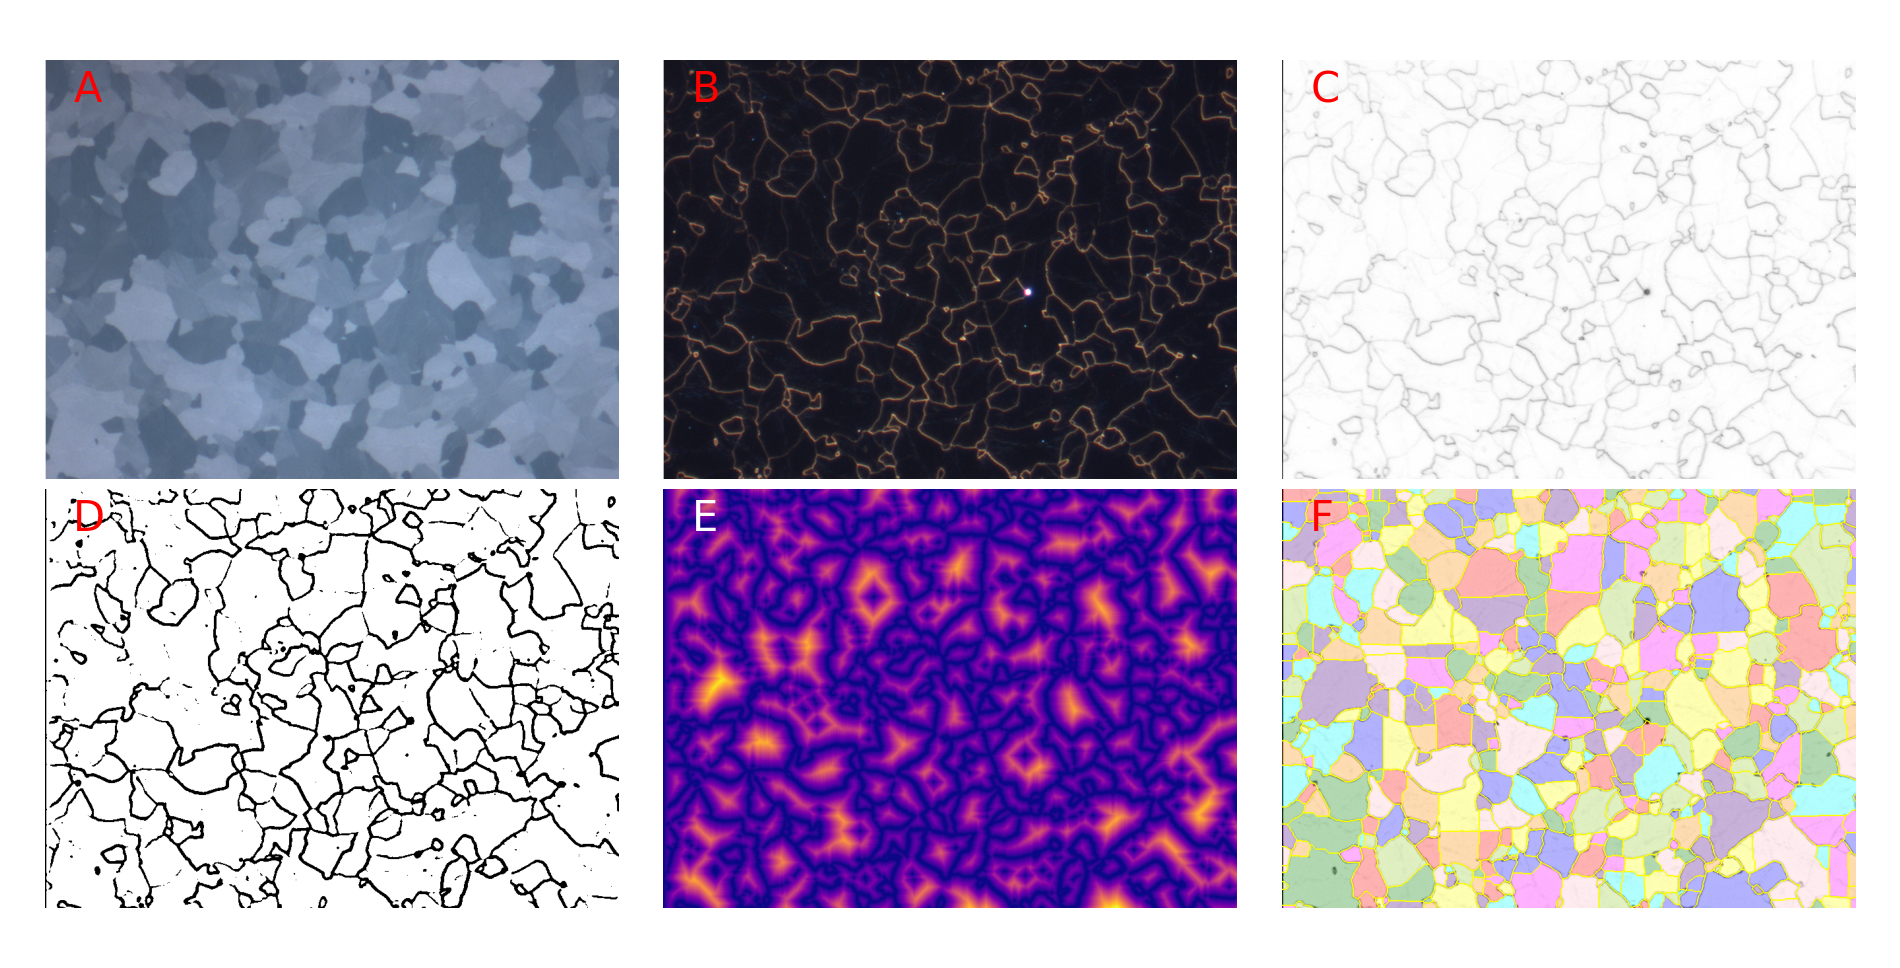
\includegraphics[width=1.0\linewidth]{microstructure_10C.png}
		\caption{}
		\label{fig:micro_10C}
	\end{figure}

	\begin{figure}[h]
		\centering
		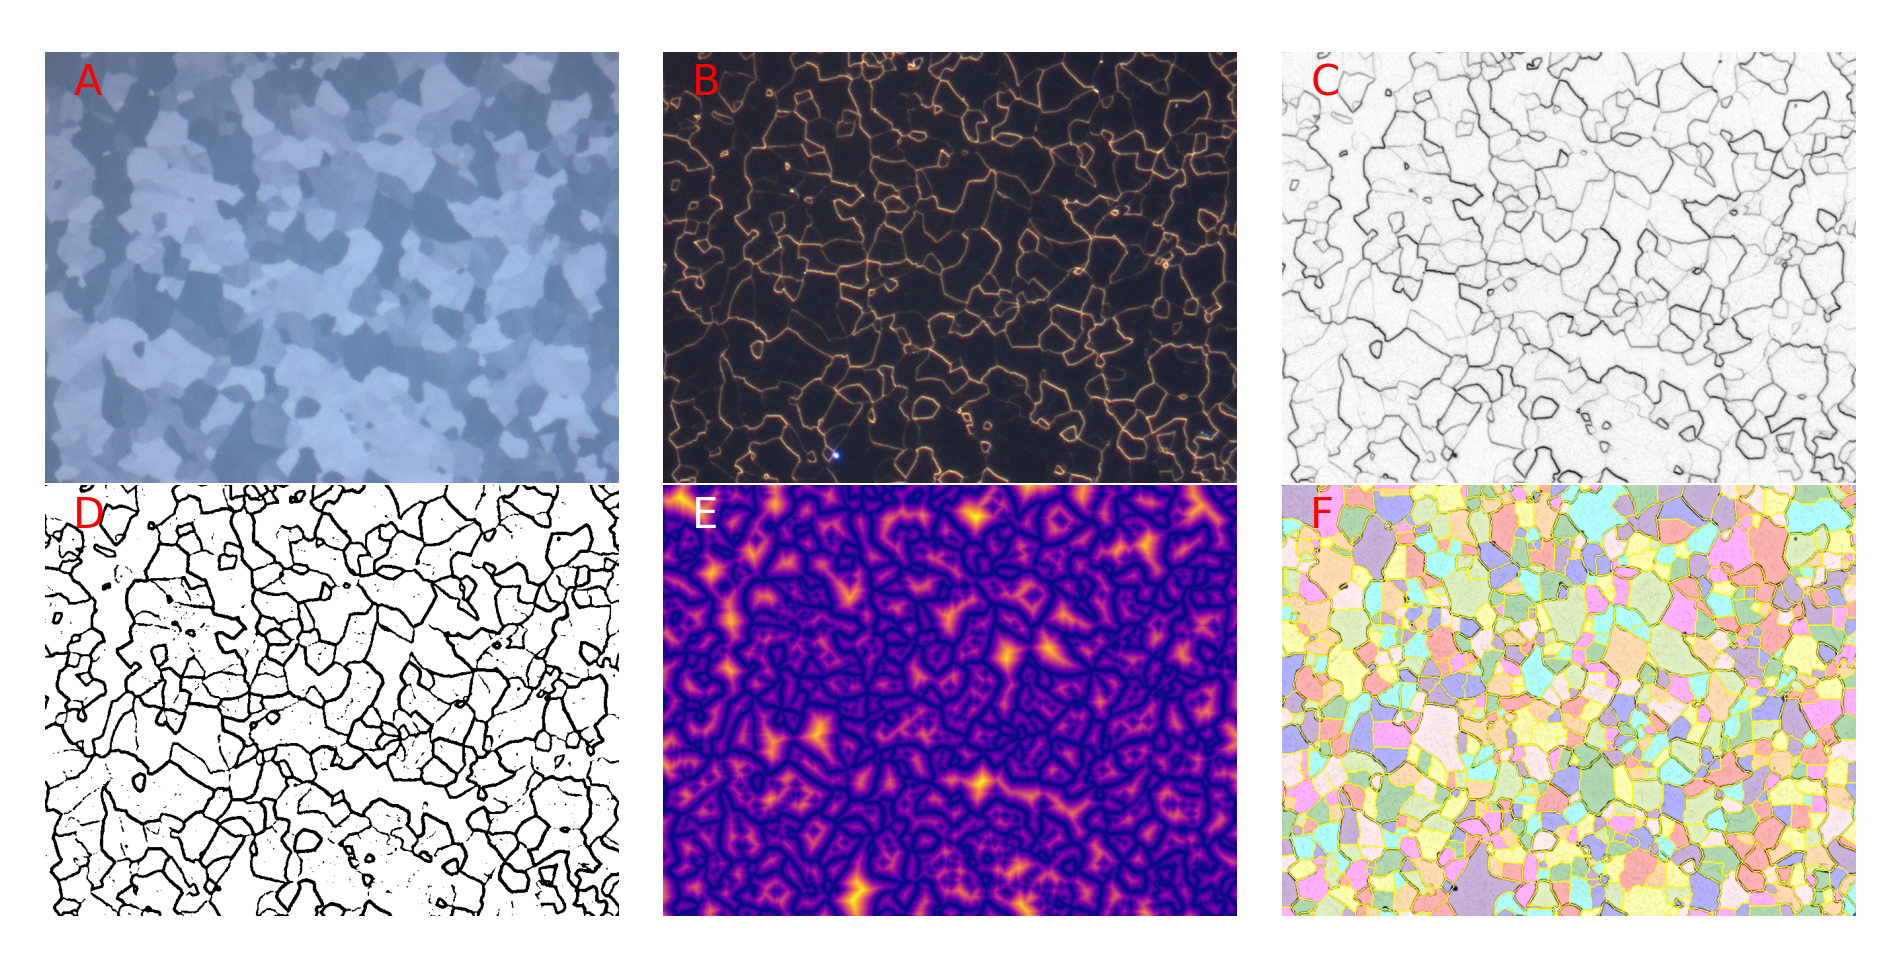
\includegraphics[width=1.0\linewidth]{microstructure_15C.png}
		\caption{}
		\label{fig:micro_15C}
	\end{figure}

	\begin{figure}[h]
		\centering
		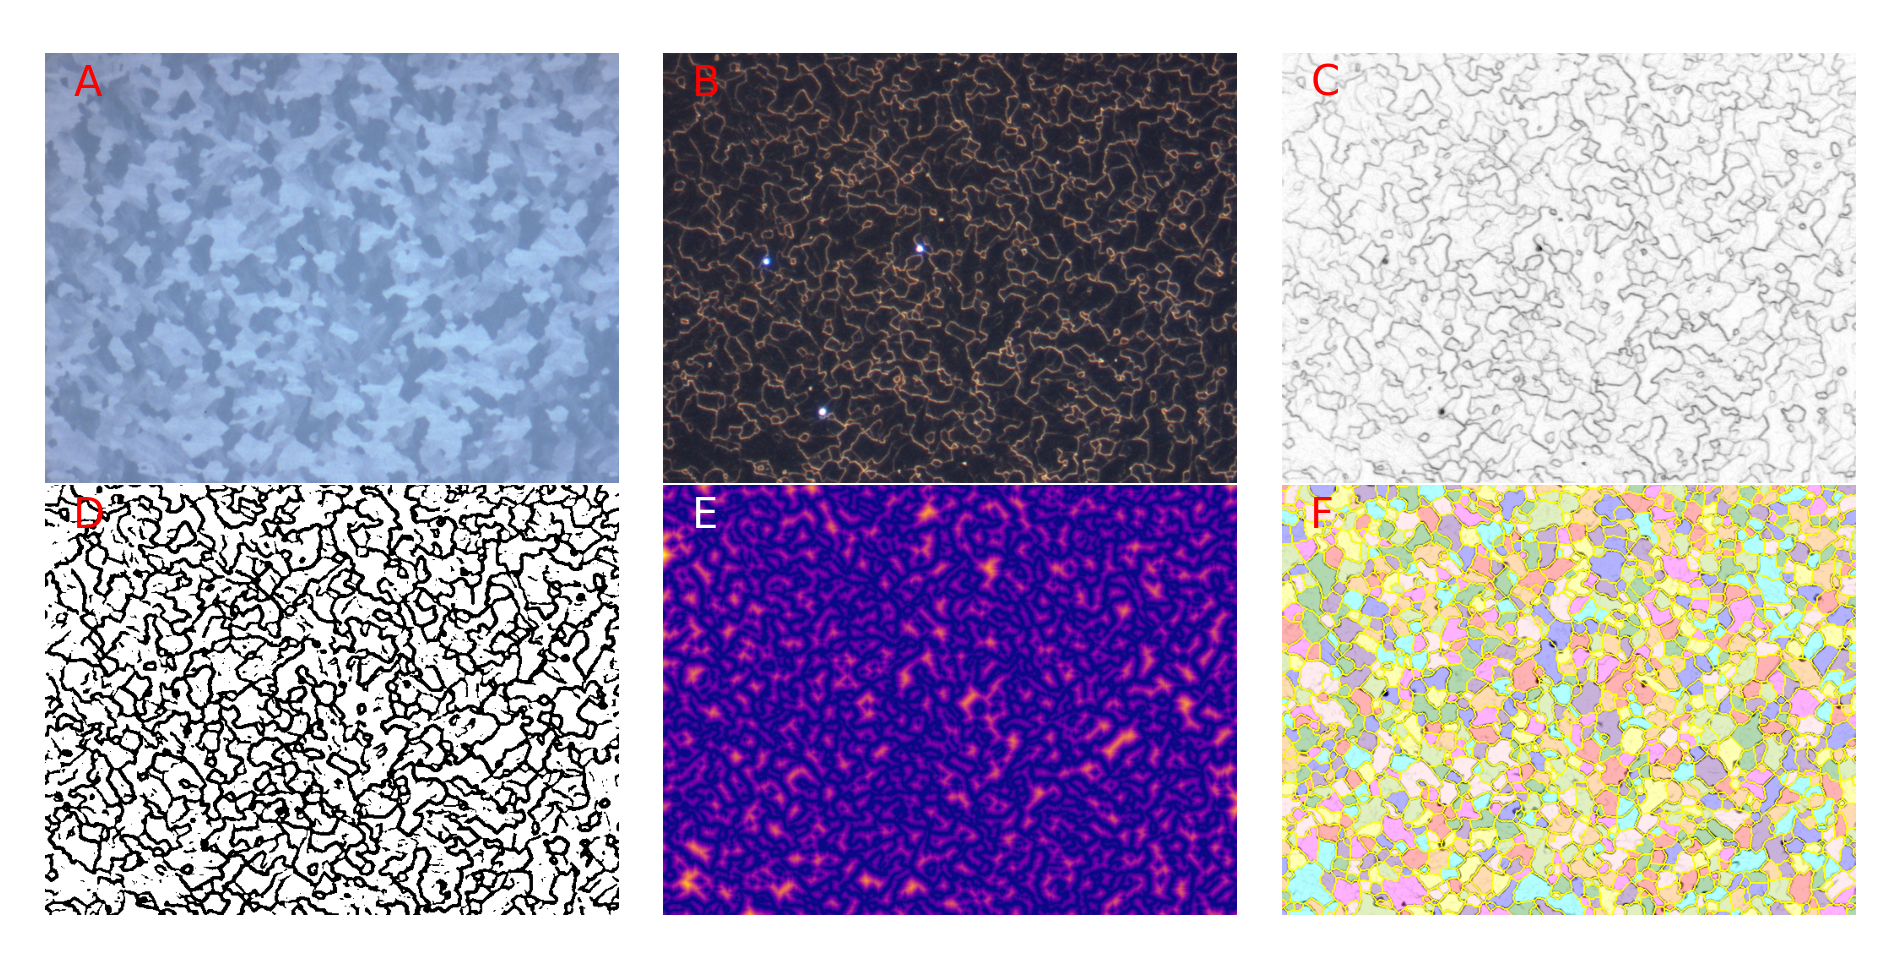
\includegraphics[width=1.0\linewidth]{microstructure_20C.png}
		\caption{}
		\label{fig:micro_20C}
	\end{figure}

	\begin{figure}[h]
		\centering
		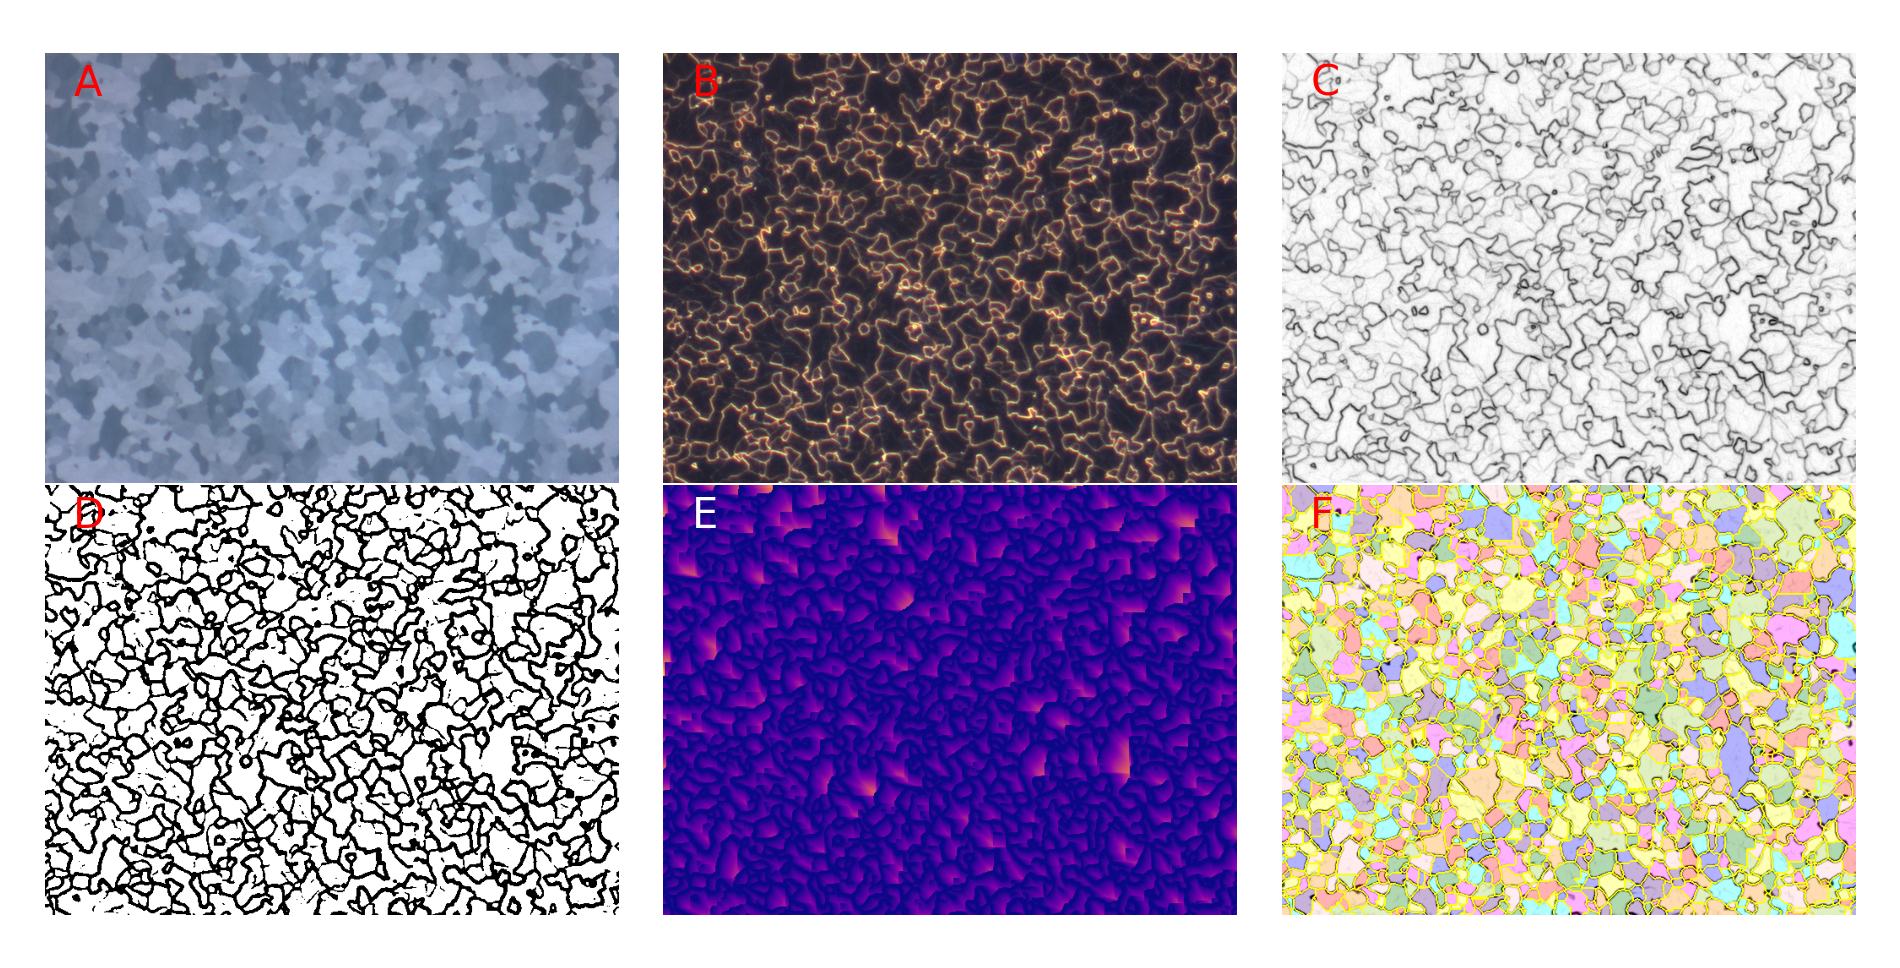
\includegraphics[width=1.0\linewidth]{microstructure_25C.png}
		\caption{}
		\label{fig:micro_25C}
	\end{figure}

	\begin{figure}[h]
		\centering
		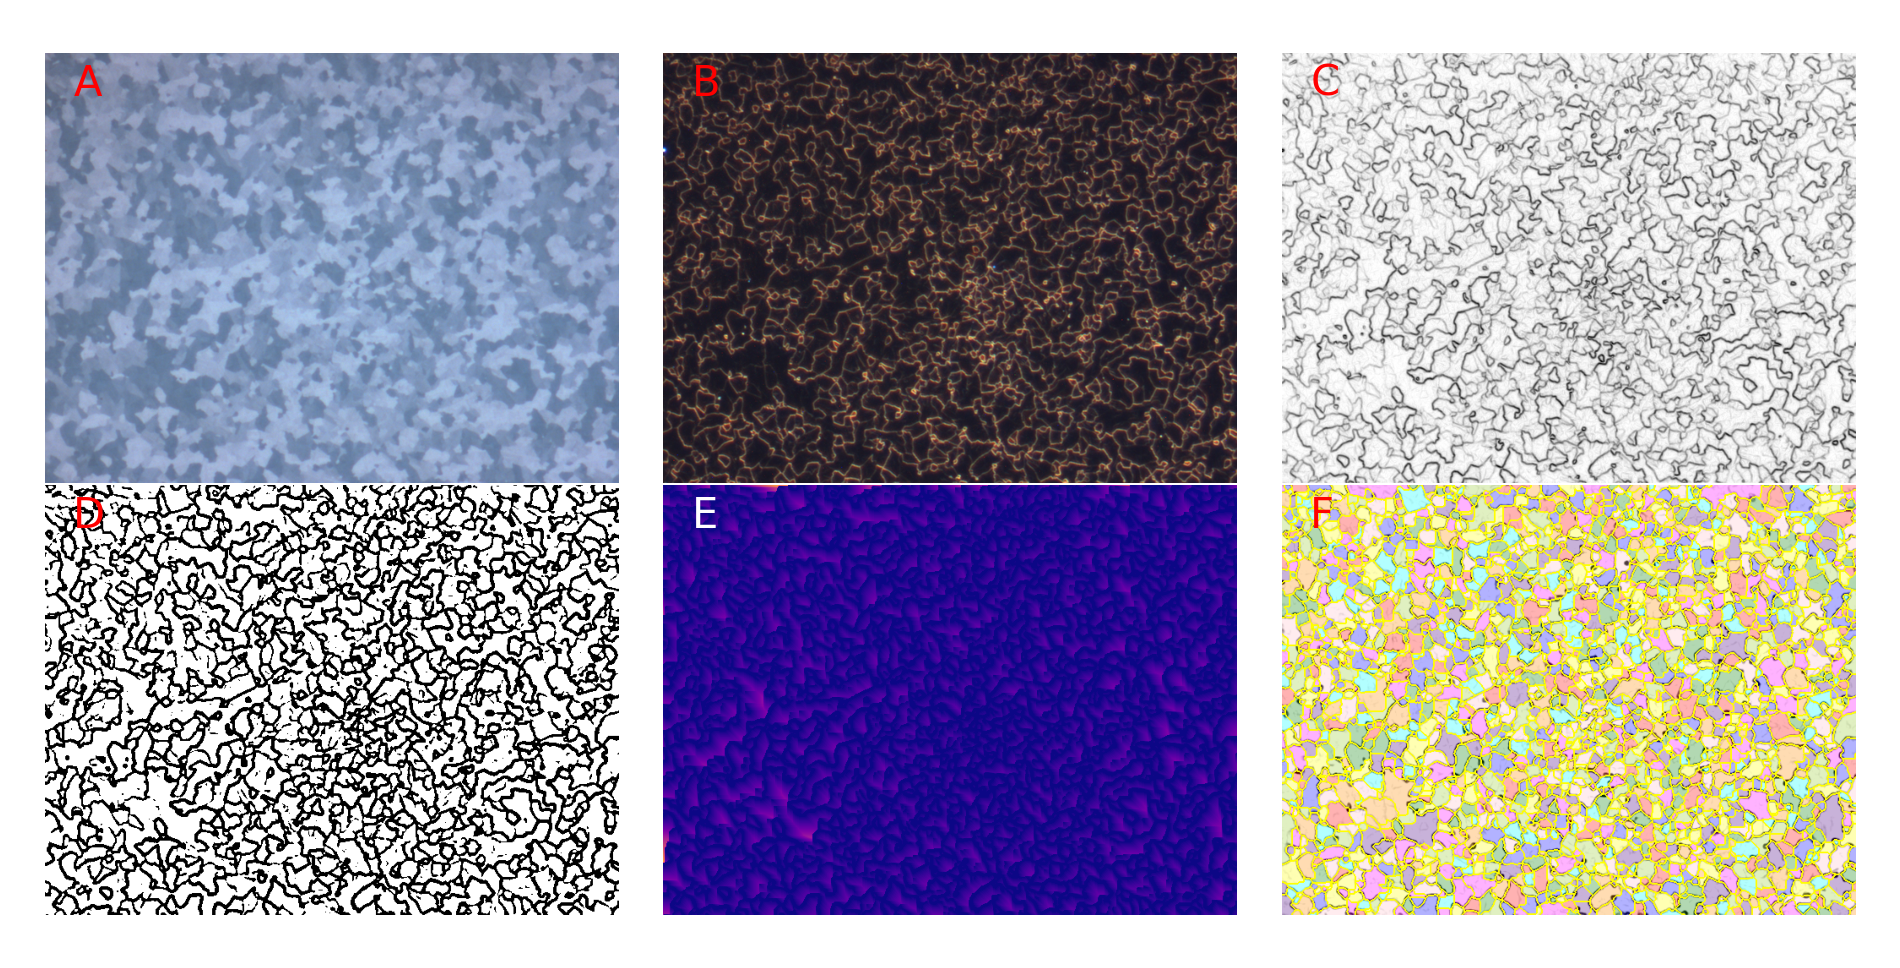
\includegraphics[width=1.0\linewidth]{microstructure_30C.png}
		\caption{}
		\label{fig:micro_30C}
	\end{figure}

	\begin{figure}[h]
		\centering
		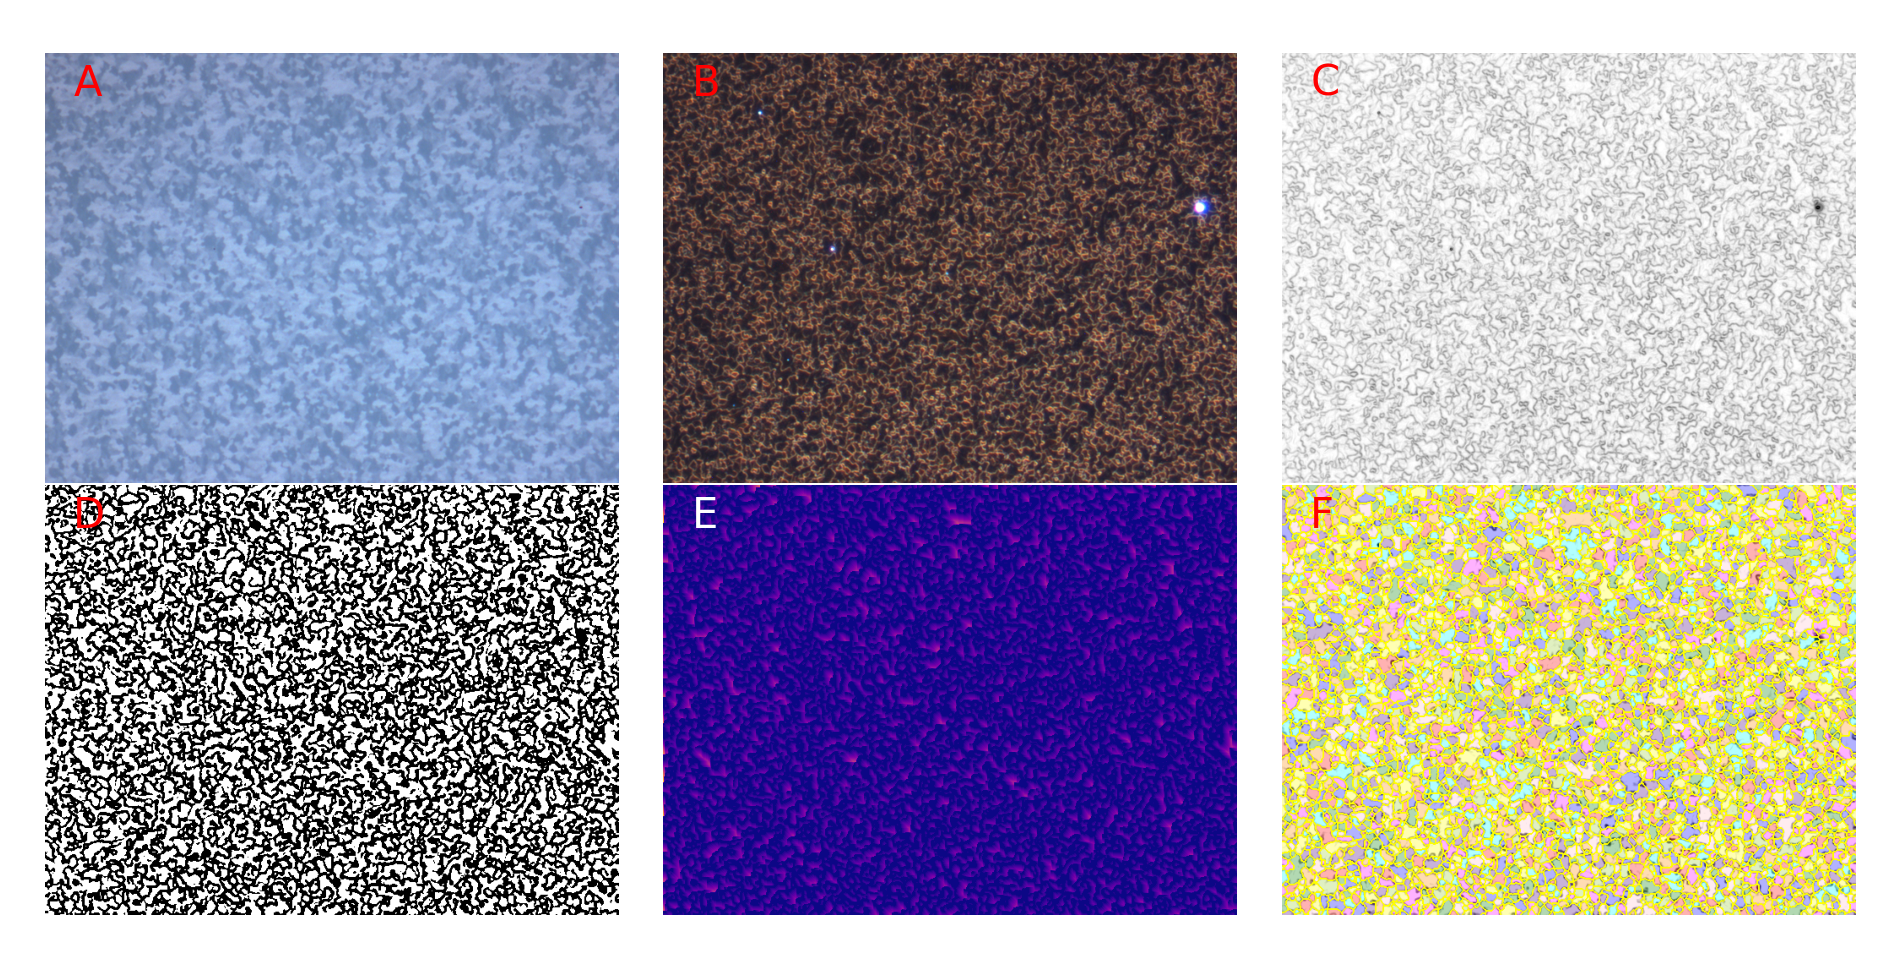
\includegraphics[width=1.0\linewidth]{microstructure_35C.png}
		\caption{}
		\label{fig:micro_25C}
	\end{figure}


\end{document}

%test\cite{chrzan:2020}
%test\cite{campbell:2018}
%test\cite{chan:2020}
%test\cite{jain:2018}
